\chapter{Concept}
In this chapter, we give a high-level overview of the different concepts and features of our proposed programming language ``Luie'' and the corresponding compiler. We also discuss some of the design decisions and draw comparisons to other programming languages targeting quantum computers. 

We start off with an overview of the language. This includes the overall structure, the different data types and statements, and some special behaviors. Next, we discuss the error handling of the compiler. There, we introduce and explain all possible warnings and critical errors that can occur. The error handling is followed by the discussion of the optimizations that the compiler may apply to the code; this includes some inherent optimizations as well as optional peephole optimizations. Lastly, we discuss the command line interface of the compiler, its options and their corresponding behavior.   

\section{Language Overview}
\begin{itemize}
    \item Given an overview of the different feature of the language
    \item How do they work and what is the reason for implementing them
    \item Why are some feature (\eg implicit iteration) \emph{not} implemented
\end{itemize}

\subsection{Blocks and Scopes}
\label{sec:concept_blocksAndScope}
Similar to many other languages, Luie uses code blocks and corresponding scopes. Both the code blocks and scopes are used to structure the code and enable the reuse of identifiers in different contexts. Each Luie program is contained in the main code block. This main code block can contain arbitrarily many other code blocks. In turn, these code blocks can also contain any number of nested blocks. However, the main code block can only exist once and is the parent block of all others. Therefore, it also cannot depend on any other block. The main block not only differs from the others in terms of hierarchy but it is also the only block that can contain composite gate definitions. The composite gates are defined at the top of the main code block and are followed by other declarations or statements. 

Similar to the main code block, all other code blocks also consist of declarations and statements. A new code block is defined either in the definition of a composite gate or in the body of a control flow primitive; this includes the if-statement, else-statement, and for-loop. Each code block has a unique scope.

Scopes represent the variable context of a code block. Since each scope corresponds to one code block, they are also hierarchically structured. In turn, the parent of a scope is the scope that directly contains this scope, while ancestors are all scopes that also indirectly contain the scope.\improvement{bad formulation}
In contrast, the descendant of a scope are all scopes that are directly and indirectly contained in the scope. Furthermore two scopes are independent if one is neither an ancestor or descendant of the other. \info{same language can be applied to code blocks} 
In a given scope, the program can access all variables previously defined in this scope and all its ancestors, however not the variables of any descendants.  
In contrast, two independent scope do not have access to the variables defined in the other scope. Therefore, two independent if-statements can define a variable with the same name in their scope. Additionally, a scope can also overwrite the definition of a variable of an ancestor with its own definition while the ancestor's definition is not affected.

\subsection{Data Types}
\label{sec:concept_dataTypes}
Luie is mainly focused on being a quantum language with quantum control flow; this is also reflected in its data types. The language operates mostly on two types of quantum data, registers and qubits. Both behave as described in Sec.~\ref{sec:background_quantumComputing} where a register represents an array of qubits with a fixed length.
\unsure{Here or in implementation: while to the outsite register array of qubits, internally qubit special case of register (with length 1).}
\dots
\begin{itemize}
    \item Different data types
    \begin{itemize}
        \item Register
        \item Qubits (Registers with size 1)
        \item Iterators, in more detail in Sec.~\ref{sec:concept_controlFlow}
    \end{itemize}
    \item How are qubits and register declared?
\end{itemize}


\subsection{Basic Operations}
\label{sec:concept_basicOperations}
\begin{itemize}
    \item Parameterized gates: p
    \item Overall universal gate set, any gate can be defined with composite gates for later use
\end{itemize}
Any language needs some basic operations to manipulate its data type. While these operations may be addition, multiplication, and similar ones, quantum computers\unsure{gate-based quantum computer, not generally} manipulate their data with gates. Luie provides multiple predefined gates with which the qubits and registers can be manipulated. The syntax for applying gates to qubits is similar to other quantum language; the name of the gate is given and all parameters are listed next, separated with commas. 

The first kind of gate set natively available are the basic single qubit gates; these include the $X$, $Y$, and $Z$ gates as well as the Hadamard gate $H$. The logical extension of single qubit gates is the second gate set, the multi-qubit gates; they include the controlled-not gate $CX$ and the Toffoli gate $CCX$. These gates are not required for the overall gate set to be universal because they can easily be simulated with the control flow abilities provided by Luie. However, they are included because most programmers are used to them.
\unsure{bad reason, write better one!}
Finally, the parameterized gates are the last gate set. In contrast to the basic single and multi-qubit gates, they are not constant in their behavior but depend on a parameter. This parameter is given as an expression and is evaluated at compile time; it is given in parenthesis after the gate itself. Currently, the only parameterized gate available is the phase gate $p(\lambda)$.
The respective behavior and mathematical definition of all predefined gates in Luie is discussed in Sec.~\ref{sec:background_quantumGates}. Since the language provides both the Toffoli and Hadamard gates, the overall gate set is universal. Furthermore, any gates that are not predefined, can easily be implemented as composite gate; they are described in Sec.\ref{ce} 

\subsection{Control Flow}
\label{sec:concept_controlFlow}
\begin{itemize}
    \item different kinds of control flow primitives
    \item qif-/else-statements
    \begin{itemize}
        \item describe
    \end{itemize}
    \item for-loops
    \begin{itemize}
        \item describe
    \end{itemize}
\end{itemize}

\subsection{Expressions}
\label{sec:concept_expressions}
The language allows for complex expression that are evaluated at compile time. These expression can be used to access specific indices of a register or define the range of a for loop. Besides the typical operations like addition and multiplication, the language also implements different functions. In the following, we want to present the operations and different functions that expressions can use, what data types they operate on, and how they behave. 

\dots
\begin{itemize}
    \item Consists of expressions, terms and factors
    \begin{itemize}
        \item Expressions consist of expression, operator, and term or just a term
        \item Term consists of term, operator, and factor or just a factor
        \item Factor consists of expression in parentheses, a negated factor, number, identifier or function call
        \item Different functions
    \end{itemize}
\end{itemize}

\subsection{Composite Gates}
\label{sec:concept_compositeGates}
\begin{itemize}
    \item Similar to composite gates in language OpenQASM
    \item Useful for gate combinations commonly used,
    \item Can also make code more readable (indirect code comments)
    \item Some significant changes
    \item Can input registers (not implicit iteration)
    \item Access to control flow statements provided by luie
    \item Example of composite gate, quantum Fourier transform depicted in Fig.~\ref{fig:qft_example}
\end{itemize}

\begin{figure}[htp]
    \centering     
    \lstinputlisting[style=Luie]{../figures/code/qft.luie}
    \caption{Luie gate definition for the Quantum Fourier Transform.}
    \label{fig:qft_example}
\end{figure}

\section{Error Handling}
Generally, an important part of a program is error handling; useful and precise error messages are essential for comfortable interactions with the program. This is especially the case for compilers where the user should not only easily understand what the issue is but also where in the source code the error occurred.  

Our compiler has two types of errors with different severities. The first type is the \emph{warning}. A warning from the compiler can indicate issues in the source code that may cause unintended behavior. However, the issue itself does not prevent the compilation of the program and is simply an indication that there may be something wrong. In contrast, the \emph{critical error} is caused by a flaw in the source program that prevents the correct compilation and will result in the abortion of the compilation. In the following, we will discuss the different warnings and critical errors the compiler may raise and their corresponding causes. Furthermore, we discuss why they are either a warning or critical error. 

\subsection{Warnings}
The compiler can throw two different kinds of warnings. The first is the invalid range warning and the second is the unused symbol warning.

An invalid range warning can occur in the context of loop statements. They iterate over a range that is defined by the user. It can be given as either a size $n$ and iterate from $0$ to $n-1$ or a start and end index, $i_{Start}$ and $i_{End}$, respectively, and iterate from the start to the end. However, the range iterator is designed to only increase. Therefore, a range where $i_{Start} \geq i_{End}$ is invalid. Since the loop statement is unrolled at compile time, a range with a size less than or equal to zero can just be ignored. However, the user may not indent this behavior. Therefore, the compiler warns the user that the range is invalid.

The unused symbol warning is raised when a symbol, \eg, a register of composite gate, is defined in the source code but never used. The unused symbol does not have any negative effect on the compilation and the optimization step can easily remove, \eg, an unused register. Therefore, this is only a warning and the program can be compiled. However, an unused symbol may indicate that the wrong symbol was used somewhere else or part of the program is no longer used. Hence, the user is warned of the unused symbol and unintended behavior may be prevented.

\subsection{Critical Errors}
The list of critical errors, often just referred to as errors, is more extensive than the list of warnings. It includes the invalid access, number of arguments for gates and functions, and size errors. Furthermore, there are errors for the attempted declaration of a variable that is already declared, an undeclared and type error, and, lastly, an error for the invalid use of a qubit in a guarded code block.

The first error is the invalid access error. It occurs when a register is accessed at an invalid index $i$, \ie, $i$ is either smaller than zero or larger than $size - 1$, where $size$ is the size of the register. While this error could easily be ignored and would cause no issue when compiling the program, the resulting code would be an invalid circuit description. 

Secondly, the invalid number of arguments error for gates and functions is caused when the number of arguments given to either a gate or function does not correspond to the number of required arguments. For example, the Hadamard gate always expects one argument while the controlled-not gate requires two. Similarly, the \texttt{sizeof}-function operates on only one argument. The compiler cannot proceed when given too few arguments; for the opposite case, while dropping any leftover arguments is possible, it would result in unexpected behavior. % Additionally, too many arguments indicate an issue in the program. 
Therefore, the compiler reports an error for both cases and aborts the compilation.

Another error is the invalid size error. It occurs then a register is declared with an invalid size. A size is invalid if it is less or equal to $0$. A register with non entries cannot be used for anything and, likely, indicates an issue in the program while a register with a negative amount of entries is impossible. Therefore the compilation is aborted and the error is thrown.

The next two errors are concerned with the declaration of variables in a given context; they are the undeclared and already-declared errors. An undeclared error is raised when a variable is used in a context where it is not defined. In this case, the symbol table does not have a symbol stored for the given identifier and the compiler cannot continue. In contrast, the already-declared error occurs when a variable is declared in a context where the same variable identifier has already been assigned to a different symbol. While the compiler could overwrite the previous declaration, this can easily lead to unexpected behavior and, in turn, we do not allow a declaration in the same scope to be overwritten. 

The type error is thrown when a variable is used in a function or gate but is not the required type. Languages with loose typing may be able to convert some types to the required type by, for example, parsing the integer value of a string. However, this can not only result in unexpected behavior and hard to debug errors in the code but, in the case of a quantum language, it may also require the conversion between classical and quantum data which is not easily achievable. 

Finally, the last error is the use-of-guard error; it occurs when a qubit is referenced in a context that is guarded by itself. While the compiler can easily translate any such occurrence, they result in a invalid circuit description. As described in Sec.~\ref{sec:background_branching}, a gate that operates on and is controlled by the same qubit cannot be reversible. Therefore, the compiler prevents the generation of an invalid circuit and aborts the compilation. 

\section{Optimization}
\label{sec:eval_optimization}
The optimizations, which are applied to the quantum circuit, are the first aspect we want to evaluate. For this, we apply our optimizations to variants of the same algorithm, the quantum ripple-carry adder. Firstly, we analyze the optimizations to the adder when given classical inputs. Next, we evaluate the optimizations of the adder for inputs in superposition with different register sizes. Lastly, we compare our optimizations to optimizations that are applied by the default Qiskit transpilation process of quantum circuits.

In our first example, we use the inputs $a = \ket{1}$ and $b = \ket{15}$, with both the input and output carry qubit having a value of $\ket{0}$. Furthermore, both input registers have a size of four qubits and, in turn, have $2^4 = 16$ possible classical values. After the adder is applied, the $a$ register and carry input, per definition, remain at their initial values of $\ket{1}$ and $\ket{0}$, respectively. In contrast, the $b$ register now has a value of $\ket{0}$ and the carry output a value of $\ket{1}$, indicating that the result of the addition is $\ket{16}$.
The quantum circuit corresponding to the example before optimization rules are applied is depicted in Fig.~\ref{fig:eval_adder_circuit}.
\begin{figure}[htp]
    \centering     
    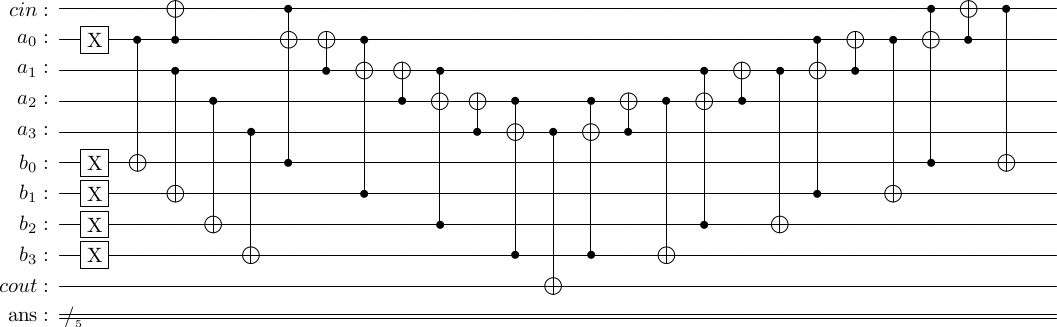
\includegraphics[width=\textwidth]{../figures/images/adderCircuit.png}
    \caption{An unoptimized circuit of a quantum ripple-carry adder.}
    \label{fig:eval_adder_circuit}
\end{figure}

Since the circuit only consists of $X$, controlled-not, and Toffoli gates, neither the Hadamard reductions nor control reversal optimization rules can be applied to the circuit. However, both the peeping control and null gate optimizations can be applied. Whenever a qubit wire contains a known value of $\ket{0}$, the controlled gates can be removed. For the opposite case, the control can be removed and the resulting $X$ gate can be removed when in combination with another $X$ gate. In turn, the circuit can be optimized such that the resulting one only contains gates that initialize the result; only two $X$ gates remain. While the first gate flips the first qubit of the $a$ register, initializing it to $\ket{1}$, the second flips the carry output qubit, indicating a result of $\ket{16}$. The OpenQASM code for the optimized circuit is depicted in App.~\ref{appendix:classicalInputs_optimized}.

In the second example, we input a value in superposition. Now, register $a$ contains a value of $\frac{1}{\sqrt{2}} (\ket{0} + \ket{3})$ and register $b$ contains a value of $\ket{4}$. Again, both carry qubits are initialized to $\ket{0}$. After the adder gate is applied, the carry qubits and register $a$ remain as initialized. However, the $b$ register now has a value of $\frac{1}{\sqrt{2}} (\ket{4} + \ket{7})$.
Since the input is now no longer a classical value, the peeping control optimization can only be applied in a few cases. In turn, only twelve gates are removed. The optimized quantum program is depicted in App.~\ref{appendix:superposInputs_optimized}. In other cases, even fewer optimizations are applied; \eg, with an input of $b = \ket{15}$, only four gates are removed while four Toffoli gates are optimized to controlled-not gates.
While the optimizations are not as effective for inputs in superposition, they can optimize significant parts of the program. For example, when we repeat both examples but increase the size of the registers to $64$ qubits, the optimized circuit contains the same amount of gates. In these cases, if qubits are not entangled by the data in superposition, all gate applications to their wires, except for the initializations, can be removed.

We also compared the optimizations applied by our compiler to the default optimizations that are applied by the Qiskit transpilation process. Qiskit\footnote{\url{https://github.com/Qiskit/qiskit/}}~\cite{JTK*24} is a software development kit for building, simulating, and transpiling quantum circuits. Additionally, the kit can interpret OpenQASM programs and build quantum circuits from them. When transpiling quantum circuits with Qiskit, \ie, transforming to a specific domain such as another basis gate set, the kit can perform optimizations to the circuit based on an optimization level. For the comparison, we used the quantum ripple-carry adder implementation provided by the OpenQASM repository\footnote{\url{https://github.com/openqasm/openqasm/blob/main/examples/adder.qasm}}. The code for the program is depicted in Fig.~\ref{fig:eval_adder_qasm}. The program can then be loaded with Qiskit and built into a quantum circuit. To apply the default optimizations of Qiskit, we transpile the circuit with the highest optimization level to the base gate set our compiler translates to, \ie, $\{X, Y, Z, CX, CCX, H\}$. While our compiler translates to arbitrary controlled gates, they are not used in this example. Furthermore, even the $Y$, $Z$, and Hadamard gates are redundant as they are not used.

\begin{figure}[htp]
    \centering     
    \lstinputlisting[style=QASM]{../figures/code/evaluation/adder.qasm}
    \caption{An OpenQASM 3 implementation of a quantum ripple-carry adder circuit.}
    \label{fig:eval_adder_qasm}
\end{figure}

However, while the Qiskit transpilation can apply many optimizations such as null gate optimizations, the default rule set does not contain a rule similar to our peeping control optimization rule. In turn, no controlled gates can be optimized in the circuit. Furthermore, since the null gate optimizations can only be applied after peeping control rules were applied, the transpilation process does not apply any optimizations to the circuit. Since Qiskit targets lower-level transpilation to specific hardware or quantum devices and not high-level optimizations, its focus is on optimizations different from ours. In contrast, our compiler has no transpilation capabilities and cannot target any specific hardware. In turn, the optimizations and overall capabilities of Qiskit and our compiler are complementary and can be used in tandem.


\section{Command Line Interface}
The command line interface of the compiler enables the programmer to interact with the compiler and specify specific behavior. There are currently four different parameters that can be specified: the input file, output file, optimizations to be applied, and the verbosity of the compilation. 

The first, and most important, parameter is the input file. Since without a specified input file the compiler has no program to compile, the parameter is mandatory. It can be given by either ``\texttt{-i}'' or ``\texttt{-{}-input}'' followed by the path to the input file. Similarly, the output file is specified with another parameter; it can be specified with ``\texttt{-o}'' or ``\texttt{-{}-output}'' followed by the path to the output file. However, this parameter is not required, and the default behavior is to create a file with the name ``output.qasm'' in the current directory.

Next, the optimization parameter can be used to specify which optimizations are applied to the code. Here, the possibilities are either none, the null gate, peeping control, Hadamard reduction, or control reversal optimization rules. Each optimization has a specific keyword that can be passed as a parameter to indicate the optimization. Additionally, multiple different optimizations can be applied by listing them separated by a plus sign.
For example, to apply both the null gate and peeping control optimizations, the correct parameter would be ``\texttt{nullgate+peepingcontrol}''. The optimization parameter is specified by either passing ``\texttt{-O}'', in this case an uppercase ``O'' to differentiate it from the output, or ``\texttt{-{}-optimization}''. When the optimization is not explicitly specified, the default behavior is no optimization. While the user can specify which optimizations are applied, they cannot specify how many optimization iterations are performed; the optimization algorithm always iterates until no further optimizations are found.

Another parameter that can be based on the compiler is the verbose parameter; it toggles the verbose mode of the compiler on. When this mode is active, the compiler prints info, warning, and error messages out to the user. In comparison, only specific error messages and warnings are displayed to the programmer when the compiler is executed without the verbose mode. In contrast to the other parameters, the verbose mode does not require any other arguments and can be activated by passing either ``\texttt{-v}'' or ``\texttt{-{}-verbose}'' to the compiler. If the parameter is not passed, the compiler is executed normally. 

Besides the parameters that can be passed to the compiler to modify its behavior, it also provides a help text. The help text can be accessed by passing the help parameter to the compiler with either ``\texttt{-h}'' or ``\texttt{-{}-help}''. Additionally, it is displayed when an invalid or unknown parameter was given by the programmer together with a message that indicates that the given parameter is invalid. The help text itself gives a short description of the compiler and lists all parameters that can be passed. Furthermore, each parameter is listed with a short description of its behavior.

An example for the usage of the CLI is depicted in Fig.~\ref{fig:concept_cli_example}. The first parameter is the input parameter; it indicates that the compiler should compile the Luie program called ``program.luie'' in the current directory. Next, the output file is specified. After the compilation is complete, the compiled code should be located in the build directory of the current directory and be called ``program.qasm''. Following the specification for the input and output files, the optimizations parameter indicates which optimizations are to be applied to the program. In this case, the compiler applies both the null gate and peeping control optimization gates. Lastly, since the verbose parameter was not specified, the compiler will only print essential errors and warnings and no other informational messages.
\begin{figure}[htp]
    \centering
    % , label=fig:concept_cli_example, caption={A command line interface example.}]
    \begin{lstlisting}[language=bash, style=bashstyle]
./LUIECompiler --input "./program.luie" 
               --output "./build/program.qasm" 
               --optimization nullgate+peepingcontrol
    \end{lstlisting}
    \caption{A command line interface example.}
    \label{fig:concept_cli_example}
\end{figure}